\documentclass[12pt]{article}

\usepackage{amsmath, mathtools}
\usepackage{amsfonts}
\usepackage{amssymb}
\usepackage{graphicx}
\usepackage{colortbl}
\usepackage{xr}
\usepackage{hyperref}
\usepackage{longtable}
\usepackage{xfrac}
\usepackage{tabularx}
\usepackage{float}
\usepackage{siunitx}
\usepackage{booktabs}
\usepackage{caption}
\usepackage{pdflscape}
\usepackage{afterpage}

\usepackage[round]{natbib}

% jen things
\usepackage[version=3]{mhchem} % electron symbol
%	\ce{n^0} \ce{e-} \ce{p+}
\usepackage{braket} % bra-ket notation
\usepackage{textcomp} % degree symbol \textdegree

%\usepackage{refcheck}

\hypersetup{
    bookmarks=true,         % show bookmarks bar?
      colorlinks=true,       % false: boxed links; true: colored links
    linkcolor=red,          % color of internal links (change box color with linkbordercolor)
    citecolor=green,        % color of links to bibliography
    filecolor=magenta,      % color of file links
    urlcolor=cyan           % color of external links
}

%% Comments

%\usepackage{color}
\usepackage[dvipsnames]{xcolor}

\newif\ifcomments\commentstrue

\ifcomments
\newcommand{\authornote}[3]{\textcolor{#1}{[#3 ---#2]}}
\newcommand{\todo}[1]{\textcolor{red}{[TODO: #1]}}
\else
\newcommand{\authornote}[3]{}
\newcommand{\todo}[1]{}
\fi

\newcommand{\wss}[1]{\authornote{blue}{SS}{#1}}
\newcommand{\an}[1]{\authornote{magenta}{Author}{#1}}
\newcommand{\meow}[1]{\authornote{Orchid}{JG}{#1}}


% For easy change of table widths
\newcommand{\colZwidth}{1.0\textwidth}
\newcommand{\colAwidth}{0.13\textwidth}
\newcommand{\colBwidth}{0.82\textwidth}
\newcommand{\colCwidth}{0.1\textwidth}
\newcommand{\colDwidth}{0.05\textwidth}
\newcommand{\colEwidth}{0.8\textwidth}
\newcommand{\colFwidth}{0.17\textwidth}
\newcommand{\colGwidth}{0.5\textwidth}
\newcommand{\colHwidth}{0.28\textwidth}

% left is what you call with latex, right is output

% Used so that cross-references have a meaningful prefix
\newcounter{defnum} %Definition Number
\newcommand{\dthedefnum}{GD\thedefnum}
\newcommand{\dref}[1]{GD\ref{#1}}
\newcounter{datadefnum} %Datadefinition Number
\newcommand{\ddthedatadefnum}{DD\thedatadefnum}
\newcommand{\ddref}[1]{DD\ref{#1}}
\newcounter{theorynum} %Theory Number
\newcommand{\tthetheorynum}{T\thetheorynum}
\newcommand{\tref}[1]{T\ref{#1}}
\newcounter{tablenum} %Table Number
\newcommand{\tbthetablenum}{T\thetablenum}
\newcommand{\tbref}[1]{TB\ref{#1}}
\newcounter{assumpnum} %Assumption Number
\newcommand{\atheassumpnum}{P\theassumpnum}
\newcommand{\aref}[1]{A\ref{#1}}
\newcounter{goalnum} %Goal Number
\newcommand{\gthegoalnum}{P\thegoalnum}
\newcommand{\gsref}[1]{GS\ref{#1}}
\newcounter{instnum} %Instance Number
\newcommand{\itheinstnum}{IM\theinstnum}
\newcommand{\iref}[1]{IM\ref{#1}}
\newcounter{reqnum} %Requirement Number
\newcommand{\rthereqnum}{P\thereqnum}
\newcommand{\rref}[1]{R\ref{#1}}
\newcounter{lcnum} %Likely change number
\newcommand{\lthelcnum}{LC\thelcnum}
\newcommand{\lcref}[1]{LC\ref{#1}}

\newcommand{\progname}{Kaplan} % PUT YOUR PROGRAM NAME HERE

\usepackage{fullpage}

\begin{document}

\title{Kaplan Software Requirements Specification for Conformer Searching} 
\author{Jen Garner}
\date{\today}
	
\maketitle

~\newpage

\pagenumbering{roman}

\section{Revision History}\label{1rev-hist}

\begin{tabularx}{\textwidth}{p{3cm}p{2cm}X}
\toprule {\bf Date} & {\bf Version} & {\bf Notes}\\
\midrule
October 4, 2018 (Thursday) & 1.0 & first draft for submission \\
\bottomrule
\end{tabularx}

~\newpage

\section{Reference Material}

Units, constants, symbols, abbreviations, and acronyms are abbreviated here, as 
used in this document.

\subsection{Table of Units and Constants}

Throughout this document SI (Syst\`{e}me International d'Unit\'{e}s) is employed
as the unit system.  In addition to the basic units, several derived units are
used as described below.  For each unit, the symbol is given followed by a
description of the unit and the SI name. Some common constants are given.
~\newline

\renewcommand{\arraystretch}{1.2}
%\begin{table}[ht]
  \noindent \begin{tabular}{l l l} 
    \toprule		
    \textbf{symbol} & \textbf{unit} & \textbf{SI}\\
    \midrule 
    \si{\metre} & length & metre\\
    \si{\angstrom} & length & $1\si{\angstrom} = 1$x$10^{-10}$\si{\metre} \\
    \si{\kilogram} & mass	& kilogram\\
    \si{\second} & time & second\\
    \si{\joule} & energy & Joule\\
    \si{\farad} & electrical capacitance & farad \\
    \si{\coulomb} & electric charge & coulomb (\si{\ampere\second}) \\
    $h$ & Planck's constant & 6.62607004x$10^{-34}$\si{\joule\second} \\
    $\hbar$ & reduced Planck's constant & $h/2\pi$\si{\joule\second} \\
    $m_e$ & mass of an electron & 9.10938x$10^{-31}$\si{\kilogram} \\
    $q_e$ & charge of an electron & 1.60217662x$10^{-19}$\si{\coulomb} \\
    $\epsilon_0$ & permittivity of free space  & 8.854187817x$10^{−12} 
    \si{\farad/\metre}$ \\
    
    \bottomrule
  \end{tabular}
  %	\caption{Provide a caption}
%\end{table}

\wss{Only include the units that your SRS actually uses}

\subsection{Table of Symbols}

The table that follows summarizes the symbols used in this document along with
their units.

\renewcommand{\arraystretch}{1.2}
%\noindent \begin{tabularx}{1.0\textwidth}{l l X}
\noindent \begin{longtable*}{l l p{12cm}} \toprule
\textbf{symbol} & \textbf{unit} & \textbf{description}\\
\midrule 

$n_a$ & unitless & number of atoms in the input molecule \\
$n_G$ & unitless & number of conformers (distinct geometries) being 
simulatenously optimised \\
$G_i$ & \si{\angstrom} & geometry for conformer $i$; matrix of cartesian 
coordinates with shape($n_a$, 3) \\
$D_i$ & \textdegree & list of dihedral angles for conformer $i$; array of 
length $n_a - 3$ \\
$E_i$ & \si{\joule} & potential energy for conformer $i$ \\
$S_E$ & \si{\joule} & sum of conformer potential energies \\
$C_E$ & $\frac{1}{\si{\joule}}$ & coefficient for $S_E$ in the fitness function 
\\
$S_{RMSD}$ & \si{\angstrom} & sum of root-mean-square distances between all 
possible combinations of conformer geometries \\
$C_{RMSD}$ & $\frac{1}{\si{\angstrom}}$ & coefficient for $S_{RMSD}$ in the 
fitness function \\
$Fit_G$ & unitless & the fitness of the set of conformers \\
$E$ & \si{\joule} & energy (of conformer) \\
$\hat{H}$ & \si{\joule} & Hamiltonian operator \\
$\Psi$ & unitless & wavefunction \\
$\sigma$ & unitless & spin ($\alpha$ or $\beta$) \\
$\phi$ & unitless & atomic orbital \\
$r$ & \si{\angstrom} & position of electron; array of length 3 \\
$R$ & \si{\angstrom} & position of nuclei; array of length 3 \\
\ce{e-} & N/A & electron \\
\bottomrule
\end{longtable*}
\wss{Use your problems actual symbols.  The si package is a good idea to use for
  units.}

\subsection{Abbreviations and Acronyms}

\renewcommand{\arraystretch}{1.2}
\begin{tabular}{l l} 
  \toprule
  \multicolumn{2}{c}{\large{Document-Specific Acronyms}} \\
  \midrule
  \textbf{Symbol} & \textbf{Description}\\
  \midrule 
  A & Assumption\\
  DD & Data Definition\\
  GD & General Definition\\
  GS & Goal Statement\\
  IM & Instance Model\\
  LC & Likely Change\\
  PS & Physical System Description\\
  R & Requirement\\
  SRS & Software Requirements Specification\\
  \progname{} & \wss{Kaplan}\\
  T & Theoretical Model\\
  \midrule
  \multicolumn{2}{c}{\large{Chemical Acronyms}} \\
  \midrule
  \textbf{Symbol} & \textbf{Description}\\
  \midrule
  BO & Bond Order \\
  SMILES & Simplified molecular-input line-entry system \\
  AO & atomic orbital \\
  MO & molecular orbital \\
  LCAO & linear combination of atomic orbitals \\
  STO & slater-type orbital \\
  GTO & gaussian-type orbital \\
  QCM & quantum chemical method \\
  BS & basis set \\
  RMSD & root-mean square deviation \\
  \bottomrule
\end{tabular}\\

\wss{Add any other abbreviations or acronyms that you add}

\newpage

\tableofcontents

~\newpage

\pagenumbering{arabic}

\section{Introduction} \label{2intro}

Molecular geometry is a necessary piece of information with regards to running 
calculations. Most computational chemists will run a geometry optimisation for 
their moleule of interest before they can investigate other properties, such as 
charge distribution and interaction energies. Without breaking any bonds, there 
are multiple ways in which the atoms can be positioned such that an optimal 
geometry is obtained - these geometries are called conformational isomers 
(sometimes abbreivated as conformers). Rather than performing an exhaustive 
search of all possible geometies, \progname{} is a package designed for the 
efficient exploration and optimisation of molecular geometry with the end goal 
of procurring a set of conformers.


\begin{figure}[H]
	\begin{center}
	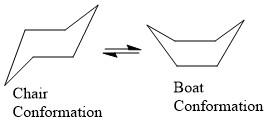
\includegraphics[]{C6H14}
	\end{center}
	\caption{Two examples of conformational isomers of cyclohexane.}
	\label{C6H14}
\end{figure}


A classic example of conformational isomers is the boat versus the chair 
conformation of cyclohexane (see Figure \ref{C6H14}). A simple geometry 
optimisation of cyclohexane would only afford the global minimum to the 
potential energy landscape, but, in using \progname{}, it will be possible to 
find the local minima of this molecule. Knowing the local minima is useful in 
areas such as drug design, where the molecule is restricted by its environment 
(for example, in the interaction with an enzyme) to have a certain shape. 
Molecules can also adopt different conformations when they are exposed to 
certain solvents, especially when the molecule in question has charge 
separation.

\wss{This SRS template is based on \citet{SmithAndLai2005, SmithEtAl2007}.  It
  will get you started, but you will have to make changes.  Any changes to
  section headings should be approved by the instructor, since that implies a
  deviation from the template.  Although the bits shown below do not include
  type information, you may need to add this information for your problem.}

\wss{Feel free to change the appearance of the report by modifying the LaTeX
  commands.}

\wss{If you are documenting a family of models, you can start from this same
  template, but you will have to add a section for variabilities.  For program
  families you should look at \cite{Smith2006, SmithMcCutchanAndCarette2017}.
  You should be able to do one document that captures the commonality analysis
  and the requirements.}

\subsection{Purpose of Document}

This document outlines the requirements that the software, \progname{}, must 
meet. It is an abstract document that does not describe the details of 
implementation. Rather, a discussion of its intended functionalities, 
performance, goals, and qualities will be presented. This document will be used 
as a reference guide when writing the software design specification and the 
software verification and validation plan. The inputs, expected outputs, and 
user characteristics for the program will be outlined, as well as the theory 
needed for searching a molecular geometry space. Any assumptions inherent to 
solving the problem will be mentioned in this document. 

\subsection{Scope of Requirements}
Kaplan will optimise the geometry of an input molecule to find its conformers 
by searching the potential energy surface. The size of molecule that can be 
accommodated depends greatly on the other inputs of the system, such as level 
of theory and convergence criteria, but should be held within reasonable bounds 
such as a maximum of a couple hundred atoms. During optimisation, the bond 
lengths and bond angles will be held fixed, and only the diehdral angles will 
be manipulated. As a result, molecules with less than 4 atoms will remain 
unchanged after optimisation (no dihedral angles). Furthermore, the conformer 
with the lowest energy is not likely to represent the true minimum of the 
potential energy landscape without subsequent optimisation of the other bond 
angles/lengths. Lastly, the system is not intended to be impervious to abnormal 
or forced bonding behaviour.

\subsection{Characteristics of Intended Reader} 
The reader should have taken first-year undergraduate chemistry, physics, and 
mathematics. They should be familiar with some bonding theory in molecules 
(valence bond (VB) theory, molecular orbital (MO) theory, and valence-shell 
electron pair repulsion (VSEPR)) and comfortable with the concept of 
optimisation (especially of a multi-dimensional surface). 

To understand the energy calculations, the reader should have taken a quantum 
physics or quantum chemistry undergraduate course. Having a basic understanding 
the following terms will be useful:
\begin{itemize}
	\item Schr\"{o}dinger equation
	\item Hartree Fock
	\item wavefunction
	\item basis set
	\item hamiltonian operator
	\item restricted versus unrestricted quantum chemistry calculations
\end{itemize}

\subsection{Organization of Document}
% TODO
This document follows the template outlined in \cite{SmithAndLai2005}. Section 
\ref{1rev-hist} provides tables for all of the units, symbols, acronyms, and 
abbreviations used throughout the document. Section \ref{2intro} is an overview 
of the purpose and scope of the system, including an explaination the intended 
reader for this document. Section \ref{3sys-desc} goes into more detail 
regarding the system and its inputs, and describes the responsibilities of the 
user versus the program. 
%TODO

\section{General System Description} \label{3sys-desc}

The interactions between the system and its environment are discussed in this 
section. The user characteristics and system constraints are also given.

\subsection{System Context}

\wss{Your system context will likely include an explicit list of user and system
  responsibilities}

Here the system context for Kaplan is shown (Figure \ref{sys-context}). With 
respect to inputs, convergence conditions includes number of expected 
conformers, energetic requirements, and the method and basis set used to 
perform energy calculations. As for ouputs, an energy will be returned for each 
conformer geometry. 

%It should be noted here that the program will not 
%calculate the energy; rather, an external library (examples: Gaussian 
%\ref{g16}, Psi4 \ref{psi4}, Horton \ref{horton}) will be called upon to do the 
%calculations. The user will not have to interact with this external library, 
%but they may have to provide input formatted to that library's specification 
%(such instructions will be included as part of Kaplan's documentation). 


\begin{figure}[H]
	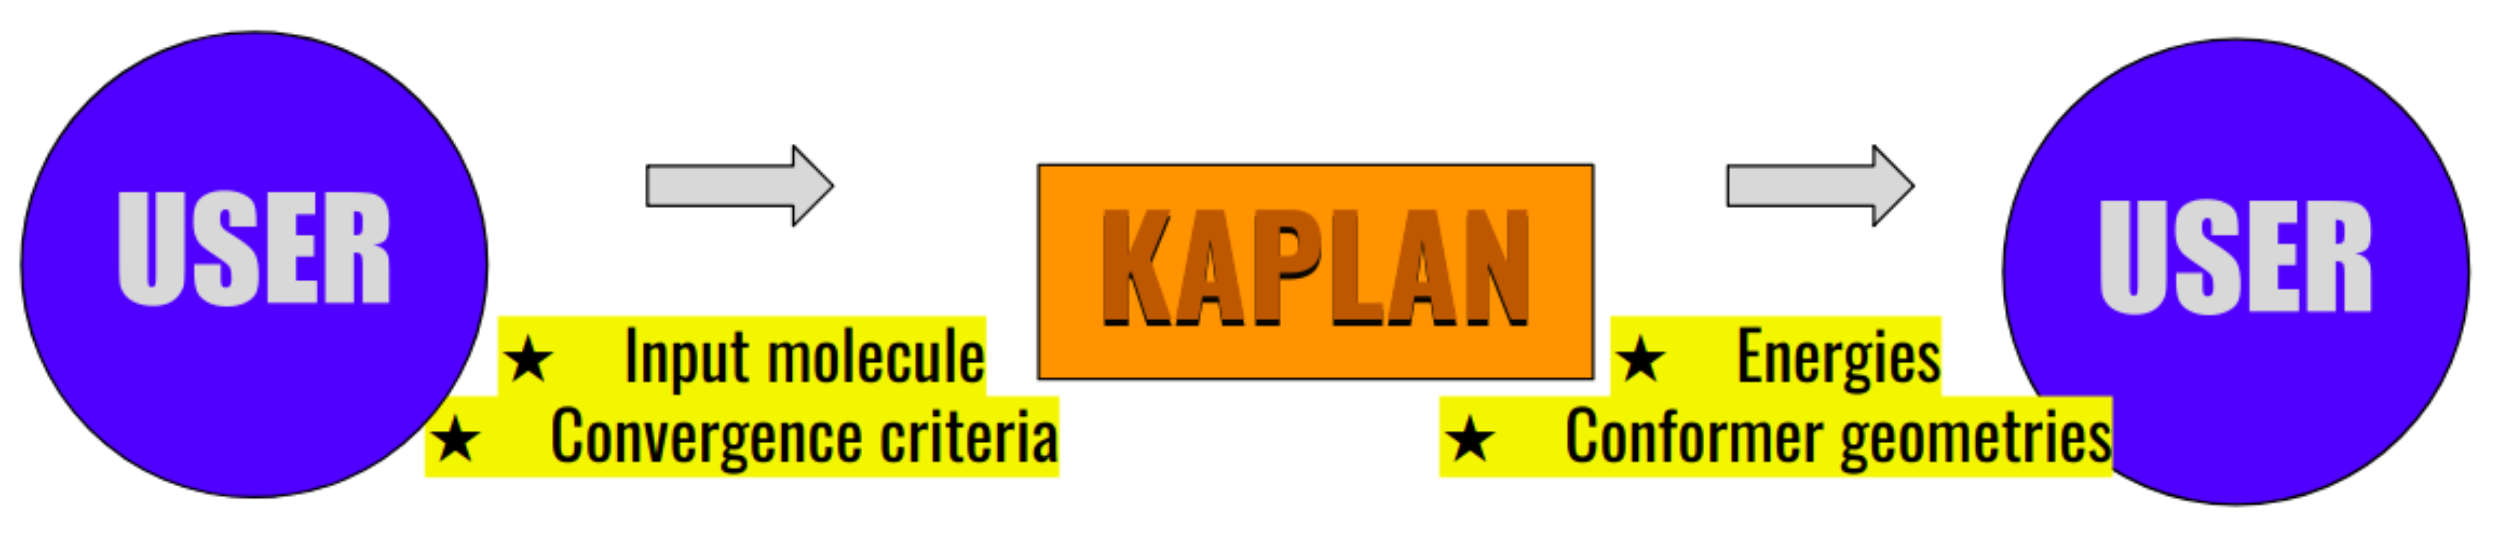
\includegraphics[width=\textwidth]{sys-context}
	\caption{The circles represent user interaction, and the rectangle 
	represents the program. The inputs are fed to the program, and the 
	outputs are given back to the user, as indicated by the arrows.}
	\label{sys-context}
\end{figure}

\begin{itemize}
\item User Responsibilities:
\begin{itemize}
\item provide chemically and computationally reasonable input

%provide an input molecule that is chemically reasonable (i.e. likely to 
%converge during optimisation)
%give a level of theory (quantum mechanical method and basis set) for 
%evaluating the energy
%\item make sure the method and basis set make chemical and computational sense 
%for the input molecule
\item set the convergence criteria (how long will the program search for 
confomers? What energetic requirements should the conformers possess? Estimate 
the number of expected conformers, etc.).
\end{itemize}
\item \progname{} Responsibilities:
\begin{itemize}
\item prepare molecular geometry for optimisation
%create initial coordinates for the molecule and generate a list of 
%dihedral angles
%convert between various input geometry types (examples: SMILES string, 
%z-matrix, xyz (cartesian) coordinates)
\item find conformers and calculate their energies
\item determine if the convergence conditions have been met
%, such as finding enough local minima (finding sufficient conformers)
\item ensure that returned conformers have distinct geometries 
\end{itemize}
\end{itemize}

\subsection{User Characteristics} \label{SecUserCharacteristics}

The user of \progname{} should have taken first year undergraduate physics, 
chemistry, and mathematics. The user must understand the 
impact of changing the quantum mechanical method and basis set for energy 
calculations, which implies that they understand basic quantum mechanics 
(including how to solve the Schr\"{o}dinger equation - 3rd year quantum physics 
course). The user should have a sense of whether their input geometry (where 
applicable) will converge under optimisation.

%They must be familiar with how to write a script such that they can interface
%with the program. 

\subsection{System Constraints}

\wss{You may not have any system constraints}
An evolutionary algorithm will be used to search the potential energy space. 
Energies will be calculated using an open-source quantum chemistry package.

\section{Specific System Description}

This section first presents the problem description, which gives a high-level
view of the problem to be solved.  This is followed by the solution 
characteristics
specification, which presents the assumptions, theories, definitions and finally
the instance models.  \wss{Add any project specific details that are relevant
  for the section overview.}

\subsection{Problem Description} \label{Sec_pd}

\wss{what problem does your program solve?}

\progname{} is designed to search the potential energy surface for 
conformational isomers of an input molecule by manipulating dihedral angles. 
The solution to a fitness function, which is related to the energies of and 
spatial differences between conformers, will be found and maximized.

\subsubsection{Terminology and Definitions}

\meow{Does the wording here imply that none of these definitions can be used in 
previous sections? Should the early sections of this document be so abstract as 
to not use any terminology?}

This subsection provides a list of terms that are used in the subsequent
sections and their meaning, with the purpose of reducing ambiguity and making it
easier to correctly understand the requirements:

\meow{Do I need to define a term if, as per the intended reader requirements, 
the reader should know what that terms means? For example, should I define 
covalent bond here?}

\begin{itemize}
\item \textbf{molecule:} a collection of atoms that are related in space, 
either covalently or non-covalently.
\item \textbf{bond angle:} the angle formed between three atoms.
\item \textbf{bond length:} the distance between the centre of masses of two 
atoms.
\item \textbf{dihedral angle} the angle between two intersecting planes, where 
each plane bisects 3 atoms.
\item \textbf{bond order:} the number of chemical bonds connecting two atoms. 
This value sometimes depends on the theory used.
\item \textbf{conformational isomer:} molecules that have the same number of 
atoms that are related by free rotation about single bonds. May also be 
referenced as conformer in the text. 
\item \textbf{quantum chemical method:} the strategies used to solve the 
Schr\"{o}dinger equation.
\item \textbf{basis set:} how to describe the molecule mathematically such that 
the Schr\"{o}dinger equation can be evaluated.
\item \textbf{z-matrix:} an input file type that uses dihedral angles and 
connectivities rather than cartesian coordinates.
\end{itemize}

\subsubsection{Physical System Description}

The physical system of \progname{} includes the following elements:

\begin{itemize}

\item[PS1:] molecule for which to find conformers. This molecule is specified 
by a file, such as xyz (cartesian coordinates) or a z-matrix, a SMILES string, 
or a name. From this geometry, the dihedral angles can be obtained.

\end{itemize}

\begin{figure}[H]
	\begin{center}
	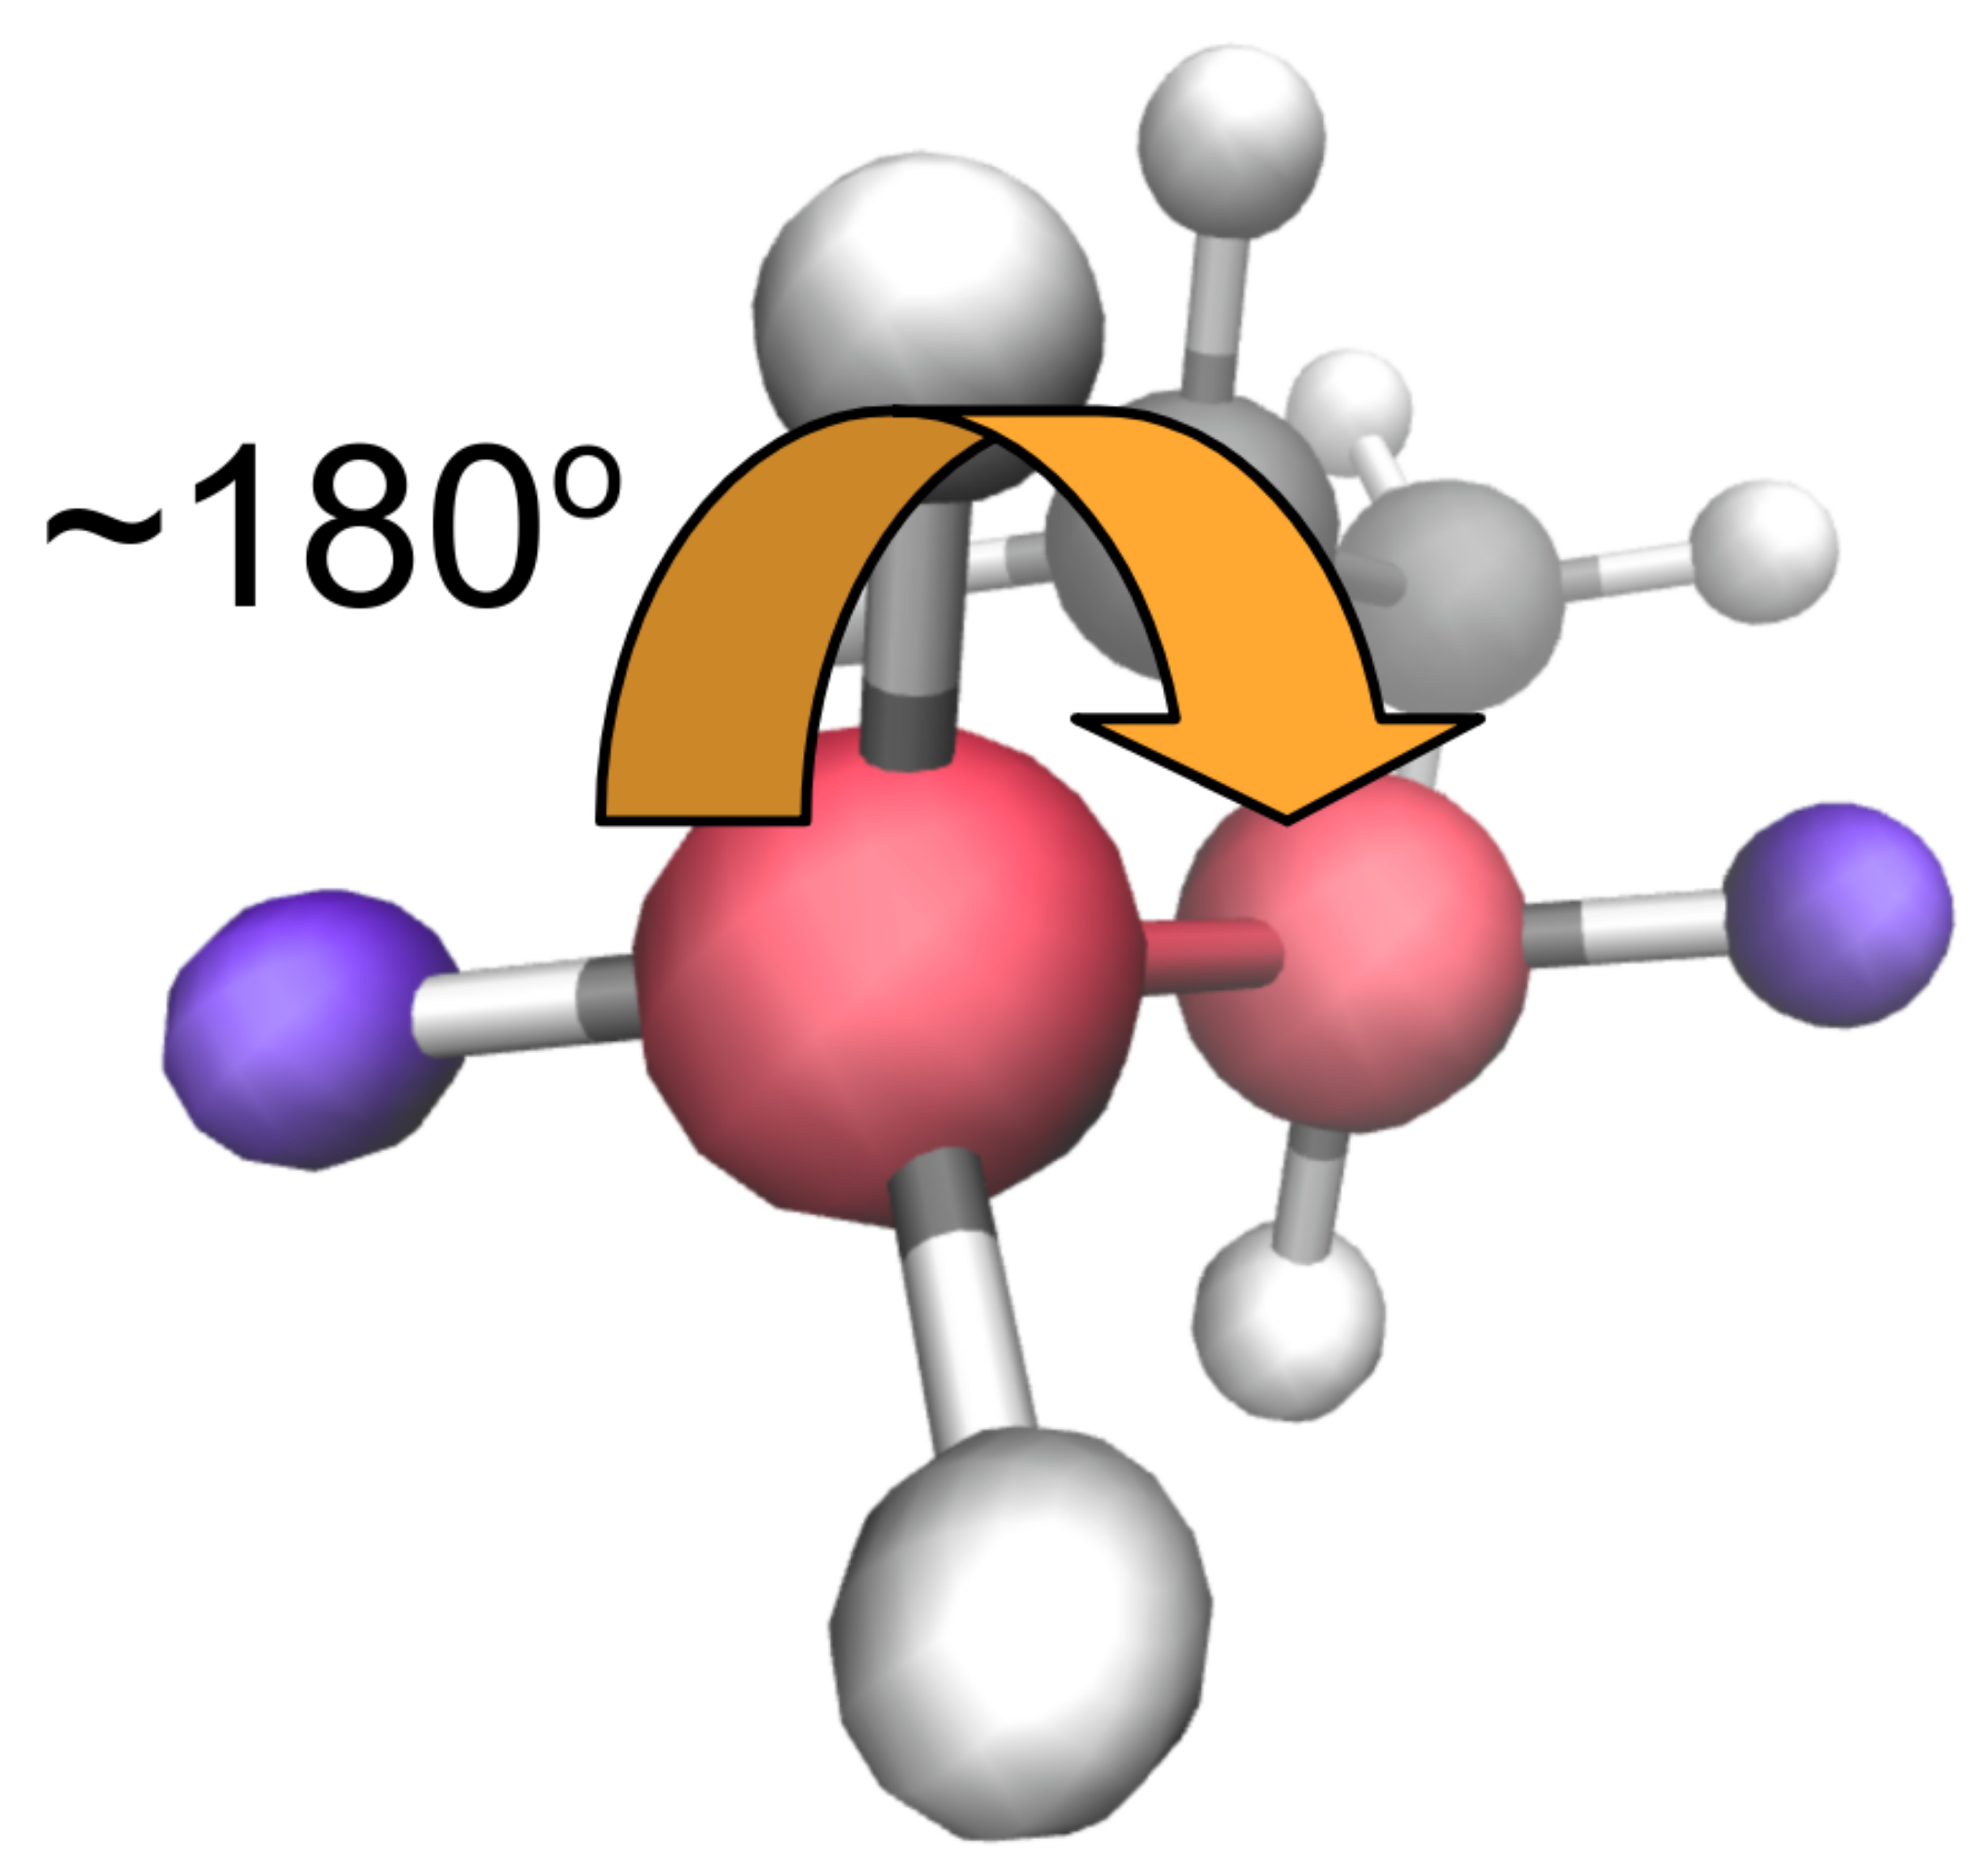
\includegraphics[width=0.5\textwidth]{butane-dihedral}
	\end{center}
	\caption{The dihedral angle formed between the 4 highlighted atoms is 
	approximately 180\textdegree. Note that if the molecule was rotated such 
	that the blue-highlighted hydrogen atom on the left went behind the 
	blue-highlighted hydrogen atom on the right, then the dihedral angle would 
	then be 0\textdegree.}
	\label{butane-dihedral}
\end{figure}

An example of the physical system for the molecule butane ($C_4H_{10}$) can be 
found in Table \ref{input-butane}.

\begin{table}[H]
	\begin{tabular}{llll}
		\toprule
		\textbf{Z-Matrix} & \textbf{XYZ (Cartesian)} & 
		\textbf{SMILES} & \textbf{Dihedral} \\
		& \textbf{Coordinates} & \textbf{String} & \textbf{Angles} \\
		\hline
	C   1 	&		14		&  CCCC & 178.8 \\
	C   1 1.527	&	butane  		&		& 238.9 \\
	C   1 1.520  2 111.489			& C -0.5630  0.5160  0.0071 &	& 121.2 \\
	C   2 1.520  1 111.497  3 178.8	& C  0.5630 -0.5159  0.0071	&	& 300.1 \\
	H   1 1.096  2 109.879  3 238.9	& C -1.9293 -0.1506 -0.0071	&	& 57.8 \\
	H   1 1.096  2 109.864  3 121.2	& C  1.9294  0.1505 -0.0071	&	& 299.7 \\
	H   2 1.096  1 109.866  3 300.1	& H -0.4724  1.1666 -0.8706	&	& 60.2 \\
	H   2 1.096  1 109.874  3  57.8	& H -0.4825  1.1551  0.8940	&	& 180.0 \\
	H   3 1.095  1 111.018  2 299.7	& H  0.4825 -1.1551  0.8940	&	& 299.7 \\
	H   3 1.095  1 110.996  2  60.2	& H  0.4723 -1.1665 -0.8706	&	& 180.0 \\
	H   3 1.095  1 110.265  2 180.0	& H -2.0542 -0.7710 -0.9003	&	& 60.2 \\
	H   4 1.095  2 111.009  1 299.7	& H -2.0651 -0.7856  0.8742	&	&	\\
	H   4 1.095  2 110.262  1 180.0	& H -2.7203  0.6060 -0.0058	&	&	\\
	H   4 1.095  2 110.989  1  60.2	& H  2.0542  0.7709 -0.9003	&	&	\\
									& H  2.7202 -0.6062 -0.0059	&	&	\\
									& H  2.0652  0.7854  0.8743	&	&	\\
	\bottomrule
	\end{tabular}
\caption{The physical system of \progname{}, using butane as an example 
molecule. The first three columns represent equivalent geometries, given in 
three different formats. The last column is the list of dihedral angles to be 
optimised by the program. During optimisation, it is important that the 
dihedral angles map back to the input geometry using the same ordering for the 
atoms.}
\label{input-butane}
\end{table}









\wss{A figure here may make sense for most SRS documents}

% \begin{figure}[h!]
% \begin{center}
% %\rotatebox{-90}
% {
%  \includegraphics[width=0.5\textwidth]{<FigureName>}
% }
% \caption{\label{<Label>} <Caption>}
% \end{center}
% \end{figure}

\subsubsection{Goal Statements}

\noindent Given an input geometry and a list of convergence criteria for a 
molecule \wss{inputs}, the goal statement is:

\begin{itemize}

\item[GS\refstepcounter{goalnum}\thegoalnum \label{goal}:] To 
create a set of conformational isomers that represent the local minima of the 
potential energy surface by optimising the molecule's dihedral angles. 
Alternatively, this GS can be described as: maximize the fitness function, 
$Fit_G$.
\wss{One sentence description of the goal.  There may be more than one.  Each 
Goal should have a meaningful label.}

\end{itemize}

\subsection{Solution Characteristics Specification}

The instance models that govern \progname{} are presented in
Subsection~\ref{sec_instance}.  The information to understand the meaning of the
instance models and their derivation is also presented, so that the instance
models can be verified.

\subsubsection{Assumptions}

This section simplifies the original problem and helps in developing the
theoretical model by filling in the missing information for the physical
system. The numbers given in the square brackets refer to the theoretical model
[T], general definition [GD], data definition [DD], instance model [IM], or
likely change [LC], in which the respective assumption is used.

  \wss{Short description of each assumption.  Each assumption
	should have a meaningful label.  Use cross-references to identify the
	appropriate traceability to T, GD, DD etc., using commands like dref, ddref 
	etc.}

\begin{itemize}

%\item[A\refstepcounter{assumpnum}\theassumpnum \label{A_meaningfulLabel}:]

%\item[A\refstepcounter{assumpnum}\theassumpnum \label{A:one-min}:] Convergence 
%can be achieved when calculating the energy of the initial geometry, however 
%specified.

\item[A\refstepcounter{assumpnum}\theassumpnum \label{A:init-params-conv}:] The 
initial bond lengths and bond angles, regardless of the type of input 
specification, will allow for the energy calculations to converge. [\tref{T_SE}]

\item[A\refstepcounter{assumpnum}\theassumpnum \label{A:E-calculable}:] The 
energy of the molecule is calculable (using quantum mechanics). [\tref{T_SE}]

\item[A\refstepcounter{assumpnum}\theassumpnum \label{A:one-min}:] The 
potential energy surface can be represented by a real-valued, continuous 
function that contains at least one minimum. [\iref{IM:fitg}]

\item[A\refstepcounter{assumpnum}\theassumpnum \label{A:emp-func}:] The 
viability of a set of conformer geometries can be evaluated by solving for the 
fitness function, $Fit_G$, whose inputs depend on the RMSD distances between 
the conformers and the energies of those conformers. A bigger value for this 
function implies a better set of conformers. 
[\iref{IM:fitg}][\ddref{Sum_E}][\ddref{Sum_RMSD}]

\item[A\refstepcounter{assumpnum}\theassumpnum \label{A:linear-fit}:] The 
fitness function is linear combination of the sum of energies and the sum of 
RMSD values. [\iref{IM:fitg}]

\item[A\refstepcounter{assumpnum}\theassumpnum \label{A:conf=min}:] Conformers 
correspond to local minima on the potential energy surface. [\iref{IM:fitg}]

\meow{A\ref{A:conf=min} might be too similar to A\ref{A:stability}.}.

\item[A\refstepcounter{assumpnum}\theassumpnum \label{A:stability}:] Within one 
potential well, the molecular geometry corresponding to a lower (more negative) 
energy will be more stable than a geometry of a higher energy. [\iref{IM:fitg}]

\item[A\refstepcounter{assumpnum}\theassumpnum \label{A:dihedral-only}:] 
Conformers can be found by manipulating dihedral angles only (i.e. bond lengths 
and bond angles will be held fixed). [\iref{IM:fitg}]

\item[A\refstepcounter{assumpnum}\theassumpnum \label{A:fixed-mol}:] The 
molecular composition does not change during the optimisation. [\tref{T_SE}]

\item[A\refstepcounter{assumpnum}\theassumpnum \label{A:one-mol}:] The 
molecule is the only calculable object in the system (no solvent, other 
molecules, etc.). This assumption does not exclude guest-host chemistry, or 
non-bonded ``molecules", from the list of permissible inputs. [\iref{IM:fitg}]

\item[A\refstepcounter{assumpnum}\theassumpnum \label{A:atom-ordering}:] The 
conformer space is independent of the ordering of the input atoms. This may 
change (subject to proof/benchmarking). [\iref{IM:fitg}]

%\item[A\refstepcounter{assumpnum}\theassumpnum \label{A:one-min}:]

\end{itemize}

\subsubsection{Theoretical Models}\label{sec_theoretical}

This section focuses on the general equations and laws that \progname{} is based
on. A quantum chemistry approach is used since this level of theory allows for 
a more accurate calculation of the molecular energy. Some assumptions are 
needed for these energy calculations in order to make the equations solvable, 
which will be discussed briefly here.

\wss{Modify the examples below for your problem, and add additional models
  as appropriate.}

~\newline

\noindent
\begin{minipage}{\textwidth}
	\renewcommand*{\arraystretch}{1.5}
	\begin{tabular}{| p{\colAwidth} | p{\colBwidth}|}
		\hline
		\rowcolor[gray]{0.9}
		Number& T\refstepcounter{theorynum}\thetheorynum \label{T_SE}\\
		\hline
		Label&\bf Non-Relativistic Time-Independent Schr\"{o}dinger Equation \\
		\hline
		Equation&  $\hat{H}\ket{\Psi} = E\ket{\Psi}$ \\
		\hline
		Description & 
		Most quantum chemical methods are focused on solving the above equation 
		for a molecule with some number of nuclei and electrons. This equation 
		is essentially an eigenvalue problem, where E gives the energy of a 
		system (the eigenvalues), $\Psi$ is the wavefunction, and $\hat{H}$ is 
		the Hamiltonian operator. An example of the electronic Hamiltonian 
		operator can be found in the Appendix (Section \ref{appendix}).\\
		\hline
		Source & \cite{szabo-ostlund} \\
		\hline
		Ref.\ By & \ddref{Sum_E}\\
		\hline
	\end{tabular}
\end{minipage}\\

The Hamiltonian, in its most explicit form, is a sum of the kinetic energies of 
the electrons ($\hat{T_e}$), the kinetic energies of the nuclei ($\hat{T_n}$), 
the electron-electron potential energy ($\hat{V_{ee}}$), the electron-nuclear 
potential energy ($\hat{V_{en}}$), and the nuclear-nuclear potential energy 
($\hat{V_{nn}}$). The potential energy terms arise from Couloumbic repulsive 
and attractive forces. The way in which the Schr\"{o}dinger equation is solved 
and how the Hamiltonian is constructed are described by the quantum chemical 
method (QCM) that is used. Some QCM examples include Hartree-Fock, 
Coupled-Cluster, Configuration-Interaction, perturbation theory, and density 
functional theory.

The Born-Oppenheimer approximation is commonly used in quantum chemical 
methods. Since the nuclei are much larger than the electrons, they move much 
more slowly. As a result, the nuclei are considered fixed and only the 
electrons move in the system. Therefore, the $\hat{T_n}$ term of the 
Hamiltonian is neglected and the $\hat{V_{nn}}$ term becomes constant. When a 
constant is added to an operator, the eigenfunctions do not change 
(wavefunction is the same). The eigenvalues (the energies) are added to the 
constant to get the final result. The electronic Hamiltonian in the 
Appendix is shown explicitly after these assumptions have been applied.

The wavefunction has no physical meaning; it is a complex-valued function for a 
single particle where the input is the position vector. The wavefunction 
squared ($|\psi(r)^2|$) is proportional to the probability of finding the 
particle at position $r = x,y,z$. That is, the integration over all space for 
$|\psi(r)^2|$ is equal to one, because the particle (if it exists) must be 
somewhere in space.

For an electron, the wavefunction describes a hydrogen atomic orbital (AO), and 
its inputs are the spin ($\sigma$) of the electron ($\alpha$ or $\beta$) and 
the position ($r$). For a multi-electron wavefunction, we have a linear 
combination of atomic orbitals (LCAO) to give the molecular orbital (MO). Since 
the number of orbitals needed to exactly describe a molecule is infinite, the 
MO is approximated by contracting the number of AO to a finite set (and thus a 
finite space), affording $\Psi(r, \sigma) = \sum\limits_{i=1}^{k}c_i 
\phi(r,\sigma)_i$, where $\phi(r,\sigma)_i$ is the AO, $c_i$ is a constant  
described by the basis set, and $k$ is the number of AO.

There are two main types of AO in quantum chemistry - Slater-type orbitals 
(STO) and Gaussian-type orbitals (GTO). STO have the form: $\phi(r,\sigma) = 
ce^{-\zeta r}$, whereas GTO have the form: $\phi(r,\sigma) = ce^{-\zeta r^2}$, 
where c is a value that depends on normalisation and the principle quantum 
number, $\zeta$ is a constant related to the effective nuclear charge, and r is 
the distance of the electron from the nucleus. STO are more accurate, have poor 
near-nuclear behaviour (approach $\infty$), but are expensive in terms of the 
evaluation of the integrals. GTO, on the other hand, are much faster to 
evaluate, but are less accurate. When a basis set is chosen for a quantum 
chemical calculation, the set of one-particle functions (AO) used to build the 
MO are described. Most quantum chemistry packages use GTO, and often the 
solution for a more accurate MO is to use a linear combination of GTO to mimic 
one STO. 

~\newline

\subsubsection{General Definitions}\label{sec_gendef}

This section collects the laws and equations that will be used in deriving the
data definitions, which in turn are used to build the instance models.
\wss{Some projects may not have any content for this section, but the section
  heading should be kept.}  \wss{Modify the examples below for your problem, and
  add additional definitions as appropriate.}

~\newline

\noindent
\begin{minipage}{\textwidth}
\renewcommand*{\arraystretch}{1.5}
\begin{tabular}{| p{\colAwidth} | p{\colBwidth}|}
\hline
\rowcolor[gray]{0.9}
Number& GD\refstepcounter{defnum}\thedefnum \label{GD_RMSD}\\
\hline
Label &\bf Root-mean square deviation \\
\hline
% Units&$MLt^{-3}T^0$\\
% \hline
SI Units&\si{\angstrom}\\
\hline
Equation&$RMSD_{ij} = \sqrt{\frac{1}{n_a}\sum\limits_{k=1}^{n_a} ((x_{ki} - 
x_{kj})^2+(y_{ki} - y_{kj})^2+(z_{ki} - z_{kj})^2)}$  \\
\hline
Description &
The root-mean square deviation ($RMSD$) is an average distance between the 
atoms of conformer $i$ and the atoms of conformer $j$. The inputs to this 
equation are the xyz coordinates for each atom (from both conformers) and the 
number of total atoms.
\\
& $n_a$ number of atoms in each conformer \\
& $x_{ki}$ the x-coordinate of the $k^{th}$ atom from conformer $i$ 
(\si{\angstrom}) 
\\
& $y_{kj}$ the y-coordinate of the $k^{th}$ atom from conformer $j$ 
(\si{\angstrom})
\\
& etc. \\
\hline
  Source & \\
  \hline
  Ref.\ By & \ddref{Sum_RMSD} \\
  \hline
\end{tabular}
\end{minipage}\\

%\subsubsection*{Detailed derivation of simplified rate of change of 
%temperature}
%
%\wss{This may be necessary when the necessary information does not fit in the
%  description field.} 

\subsubsection{Data Definitions}\label{sec_datadef}

This section collects and defines all the data needed to build the instance
models. The dimension of each quantity is also given.  \wss{Modify the examples
  below for your problem, and add additional definitions as appropriate.}

~\newline

\noindent
\begin{minipage}{\textwidth}
	\renewcommand*{\arraystretch}{1.5}
	\begin{tabular}{| p{\colAwidth} | p{\colBwidth}|}
		\hline
		\rowcolor[gray]{0.9}
		Number & DD\refstepcounter{datadefnum}\thedatadefnum \label{Sum_E}\\
		\hline
		Label & \bf Sum of conformer energies\\
		\hline
		Symbol & $S_E$\\
		\hline
		% Units& $Mt^{-3}$\\
		% \hline
		SI Units & \si{\joule}\\
		\hline
		Equation & $\left|\sum\limits_{i=1}^{G_n}E_i\right|$ \\
		\hline
		Description & 
		$E_i$ is the energy (\si{\joule}) of conformer $i$, as calculated by 
		solving the Schr\"{o}dinger equation (T\ref{T_SE}), and $G_n$ is the 
		number of conformers being simultaneously optimised by the system. The 
		individual energies should be negative; the absolute value bars imply 
		that, when this summation is included in the overall fitness function, 
		we are maximising the value of the fitness function.
		\\
		\hline
		Sources& N/A \\
		\hline
		Ref.\ By & \iref{IM:fitg}\\
		\hline
	\end{tabular}
\end{minipage}\\

\noindent
\begin{minipage}{\textwidth}
	\renewcommand*{\arraystretch}{1.5}
	\begin{tabular}{| p{\colAwidth} | p{\colBwidth}|}
		\hline
		\rowcolor[gray]{0.9}
		Number & DD\refstepcounter{datadefnum}\thedatadefnum \label{Sum_RMSD}\\
		\hline
		Label & \bf Sum of root-mean square deviations \\
		\hline
		Symbol & $S_{RMSD}$\\
		\hline
		% Units& $Mt^{-3}$\\
		% \hline
		SI Units & \si{\angstrom}\\
		\hline
		Equation & $\sum\limits_{i\neq j}RMSD_{ij}$ \\
		\hline
		Description & 
		$RMSD_{ij}$ is the root-mean square deviation between conformers $i$ 
		and $j$ (\si{\angstrom}), as calculated by using the distance formula 
		given in \dref{GD_RMSD}. This 
		distance represents how different two conformer geometries are from one 
		another on average.
		\\
		\hline
		Sources& N/A \\
		\hline
		Ref.\ By & \iref{IM:fitg}\\
		\hline
	\end{tabular}
\end{minipage}\\

\subsubsection{Instance Models} \label{sec_instance}    

This section transforms the problem defined in Section~\ref{Sec_pd} into 
one which is expressed in mathematical terms. It uses concrete symbols defined 
in Section~\ref{sec_datadef} to replace the abstract symbols in the models 
identified in Sections~\ref{sec_theoretical} and~\ref{sec_gendef}.

The goal \gsref{goal} \wss{reference your goals} is solved by \iref{IM:fitg} 
\wss{reference your instance
  models}. \iref{IM:fitg} is an empirical function designed to explore the 
  potential energy space for a molecule. Given a multi-variate surface that 
  depends on dihedral angles, manipulate those dihedral angles and solve for 
  $Fit_G$. This fitness function has two arbitrary coefficients, $C_E$ and 
  $C_{RMSD}$ that the user must determine through experimentation with their 
  molecule. \wss{other details, with 
  cross-references where appropriate.}
\wss{Modify the examples below for your problem, and add additional models as
  appropriate.}

~\newline

%Instance Model 1

\noindent
\begin{minipage}{\textwidth}
\renewcommand*{\arraystretch}{1.5}
\begin{tabular}{| p{\colAwidth} | p{\colBwidth}|}
  \hline
  \rowcolor[gray]{0.9}
  Number& IM\refstepcounter{instnum}\theinstnum \label{IM:fitg}\\
  \hline
  Label& \bf Fitness of conformer geometries $Fit_G$\\
  \hline
  Input&$C_E$, $C_{RMSD}$, $S_E$, $S_{RMSD}$ \\
  & The input is constrained so that $C_E > 0$ and $C_{RMSD} > 0$\\
  \hline
  Output&$Fit_G = C_E S_E + C_{RMSD} S_{RMSD}$ \\
  & This equation is entirely empirical and its output does not have any 
  physical meaning. The purpose of the equation is to represent the optimal set 
  of conformers for a given input molecule.\\
  \hline
  Description&$C_E$ is the energy coefficient water temperature 
  (\si{1/\joule}).\\
  &$S_E$ is the absolute value of the sum of conformer energies (\ddref{Sum_E}) 
  (\si{\joule}).\\
  &$C_{RMSD}$ is root-mean square deviation coefficient (\si{1/\angstrom}).\\
  &$S_{RMSD}$ is sum of root-mean square deviations for each conformer 
  (\ddref{Sum_RMSD}) (\si{\angstrom}).\\
  & The above equation applies when the number of conformers is greater than 1. 
  If the number of conformers is exactly one, then the $RMSD$ terms should be 
  set to zero.
  \\
  \hline
  Sources& N/A \\
  \hline
  Ref.\ By & None \\
  \hline
\end{tabular}
\end{minipage}\\

%~\newline

%\subsubsection*{Derivation of ...}
%
%\wss{May be necessary to include this subsection in some cases.}

\subsubsection{Data Constraints} \label{sec_DataConstraints}    

Tables~\ref{TblInputVar} and \ref{TblOutputVar} show the data constraints on the
input and output variables, respectively.  The column for physical constraints gives
the physical limitations on the range of values that can be taken by the
variable.  The column for software constraints restricts the range of inputs to
reasonable values.  The constraints are conservative, to give the user of the
model the flexibility to experiment with unusual situations.  The column of
typical values is intended to provide a feel for a common scenario, but for 
this project the typical values are very specific to the input geometry.  The
uncertainty column provides an estimate of the confidence with which the
physical quantities can be measured.  This information would be part of the
input if one were performing an uncertainty quantification exercise.

The specification parameters in Table~\ref{TblInputVar} are listed in
Table~\ref{TblSpecParams}.

\meow{There is no associated uncertainty with any of my values. Also, in most 
cases the typical values will be specific to the molecule (specifically, number 
of atoms). Should these two columns still be in this table?}

For $C_E$ and $C_{RMSD}$, the values for the coefficients depend on the shape 
of the potential energy surface. For example, in a surface where the minima are 
close together and the potential wells for the conformers are very high, 
placing more emphasis on $C_E$ (i.e. making $C_E$ bigger) would enable a better 
$Fit_G$. In the case where there are many low-lying conformers with wide energy 
basins, then the emphasis on $C_{RMSD}$ would afford a better result. The 
number of conformers may not be known at the start of the program; the user may 
have to determine this value through experimentation with the code.

\begin{table}[!h]
  \caption{Input Variables} \label{TblInputVar}
  \renewcommand{\arraystretch}{1.2}
\noindent \begin{longtable*}{l l l l c} 
  \toprule
  \textbf{Var} & \textbf{Physical Constraints} & \textbf{Software Constraints} &
                             \textbf{Typical Value} & \textbf{Uncertainty}\\
  \midrule 
  $G_n$ & $n\geq 2\text{*} | n\in{\mathbb{Z}}$ & $G_n \leq G_{max}$ & 2-5 & N/A 
  \\
  $C_E$ & $C_E > 0$ & $C_E > 0$ & 0.5 & N/A \\
  $C_{RMSD}$ & $C_{RMSD} > 0$ & $C_{RMSD} > 0$ & 0.5 & N/A \\
  $BS$ & available for molecule & available in software package & cc-pVTZ & N/A 
  \\
  $QCM$& available for molecule & available in software package & CCSD & N/A \\
  \bottomrule
\end{longtable*}
\end{table}

\noindent 
\begin{description}
\item[(*)] if $G_n$ is equal to one, then the $Fit_G$ function should be 
changed to only consider the energy term and not the RMSD term. \wss{you might 
need to add some notes or clarifications}
\end{description}

\begin{table}[!h]
\caption{Specification Parameter Values} \label{TblSpecParams}
\renewcommand{\arraystretch}{1.2}
\noindent \begin{longtable*}{l l} 
  \toprule
  \textbf{Var} & \textbf{Value} \\
  \midrule 
  None & - \\
  \bottomrule
\end{longtable*}
\end{table}

\begin{table}[!h]
\caption{Output Variables} \label{TblOutputVar}
\renewcommand{\arraystretch}{1.2}
\noindent \begin{longtable*}{l l} 
  \toprule
  \textbf{Var} & \textbf{Physical Constraints} \\
  \midrule 
  $Fit_G$ & $Fit_G > 0$
  \\
  \bottomrule
\end{longtable*}
\end{table}

\subsubsection{Properties of a Correct Solution} \label{sec_CorrectSolution}

\noindent
A correct solution must exhibit \wss{fill in the details}

\section{Requirements}

This section provides the functional requirements, the business tasks that the
software is expected to complete, and the nonfunctional requirements, the
qualities that the software is expected to exhibit.

\subsection{Functional Requirements}




\noindent \begin{itemize}

\item[R\refstepcounter{reqnum}\thereqnum \label{R_Inputs}:] Input the following 
parameters for the molecule whose conformers should be found. The molecule can 
be given as a SMILES string (example: ``C[N]1C=NC2=C1C(N(C(N2C)=O)C)=O''), name 
(example: ``caffeine''), xyz coordinates file, or z-matrix file. For example, 
the pubchem database can be queried with a name and is able to return 3D 
coordinates for that molecule. The other inputs that are required include the 
basis set and method; these inputs specify exactly how the Schr\"{o}dinger 
Equation (\tref{T_SE}) should be solved in order to get the energy. See Table 
\ref{input-butane} for an example of what these molecular specifications look 
like. \wss{Requirements for the inputs that are supplied by the user.  This 
information has to be explicit.}

\begin{tabularx}{\textwidth}{p{1.7cm}p{2cm}p{2cm}X}
	\toprule
	symbol & unit & data type & description \\
	\midrule
	$G_n$ & unitless & integer & number of conformers (distinct geometries) 
	to search for \\
	$C_E$ & \si{\joule} & floating point & coefficient for energy term in 
	fitness function \\
	$C_{RMSD}$ & \si{\metre} & floating point & coefficient for RMSD term 
	in fitness function \\
	BS & unitless & string & basis set \\
	QCM & unitless & string & quantum chemical method \\
	molecular geometry & \si{\angstrom}, \textdegree & file, string & name, 
	SMILES 
	string, xyz file, z-matrix file - a way to specify to connectivity of 
	the input molecule \\
	\bottomrule
\end{tabularx}

\item[R\refstepcounter{reqnum}\thereqnum \label{R_OutputInputs}:] Given the 
inputs from \rref{R_Inputs}, use \iref{IM:fitg} to solve for $Fit_G$. Based on 
the initial geometry, generate a set of random dihedral angles $D_i$, whose 
size should be equal to $n_G$.
	\wss{It 
isn't
    always required, but often echoing the inputs as part of the output is a
    good idea.}

\item[R\refstepcounter{reqnum}\thereqnum \label{R_Calculate}:] Calculate the 
energy $E_i$ for each conformer and the RMSD distance between each conformer 
pair and use these values to solve for \iref{IM:fitg}. \wss{Calculation
    related requirements.}

\item[R\refstepcounter{reqnum}\thereqnum \label{R_VerifyOutput}:] Verify that 
the energy calculations converge (\aref{A:init-params-conv}, 
\aref{A:E-calculable}) and that $Fit_G$ satisfies 
the requirement in 
Table \ref{TblOutputVar}.
  \wss{Verification related requirements.}

\item[R\refstepcounter{reqnum}\thereqnum \label{R_Output}:] Convert the 
dihedral angles $D_i$ for each conformer back to a xyz geometry (using 
\aref{A:dihedral-only}, \aref{A:atom-ordering}). \wss{Output related
    requirements.}

\end{itemize}

\subsection{Nonfunctional Requirements}

\wss{List your nonfunctional requirements.  You may consider using a fit
  criterion to make them verifiable.}
Given that the fitness function is empirical, \progname{} should be relatively 
robust with regards to changes made to the definition of $Fit_G$.
Maintainability is also important for other students who will use the project 
later-on. The program should be parallelisable and capable of running on 
high-performance computing servers without a difficult install process 
(usability, portability). The program should have some suggestions for inputs 
(example, default values for $n_G$, $C_E$, and $C_{RMSD}$) to help the user get 
started. The program should work well with other quantum chemistry packages.

\section{Likely Changes}    

\noindent \begin{itemize}

\item[LC\refstepcounter{lcnum}\thelcnum\label{LC_linear-fit}:] The assumption 
that the fitness function is linear with respect to energies and distances has 
not been verified; the function could be exponential, sinusoidal, etc.
\aref{A:linear-fit}. \wss{Give
    the likely changes, with a reference to the related assumption (aref), as 
    appropriate.}

\item[LC\refstepcounter{lcnum}\thelcnum\label{LC_indep-ordering}:] The 
assumption that the ordering of the atoms does not change the conformer space 
has not been verified \aref{A:atom-ordering}.

\end{itemize}

\section{Traceability Matrices and Graphs}

The purpose of the traceability matrices is to provide easy references on what
has to be additionally modified if a certain component is changed.  Every time a
component is changed, the items in the column of that component that are marked
with an ``X'' may have to be modified as well. 


% Table~\ref{Table:trace} shows the
%dependencies of theoretical models, general definitions, data definitions, and
%instance models with each other. Table~\ref{Table:R_trace} shows the
%dependencies of instance models, requirements, and data constraints on each
%other. Table~\ref{Table:A_trace} shows the dependencies of theoretical models,
%general definitions, data definitions, instance models, and likely changes on
%the assumptions.

\wss{You will have to modify these tables for your problem.}

%\afterpage{
%\begin{landscape}
\begin{table}[h!]
\centering
\label{Table:A_trace}
\begin{tabular}{|c|c|c|c|c|c|c|c|c|c|c|c|}
\hline
	& \aref{A:init-params-conv} 
	& \aref{A:E-calculable}
	& \aref{A:one-min}
	& \aref{A:emp-func}
	& \aref{A:linear-fit}
	& \aref{A:conf=min}
	& \aref{A:stability}
	& \aref{A:dihedral-only}
	& \aref{A:fixed-mol}
	& \aref{A:one-mol}
	& \aref{A:atom-ordering} \\
\hline
\tref{T_SE}               &X&X& & & & & & &X& & \\ \hline
\ddref{Sum_E}             & & & &X& & & & & & & \\ \hline
\ddref{Sum_RMSD}          & & & &X& & & & & & & \\ \hline
\dref{GD_RMSD}            & & & & & & & & & & & \\ \hline
\iref{IM:fitg}            & & & &X&X&X&X&X& &X&X\\ \hline
\lcref{LC_linear-fit}     & & & & &X& & & & & & \\ \hline
\lcref{LC_indep-ordering} & & & & & & & & & & &X\\ \hline
\end{tabular}
\caption{Traceability Matrix Showing the Connections Between Assumptions and Other Items}

\end{table}
%\end{landscape}
%}



\begin{table}[H]
	\centering
	\label{Table:trace}
	\begin{tabular}{|c|c|c|c|c|c|}
		\hline        
		& \tref{T_SE} 
		& \ddref{Sum_E}
		& \ddref{Sum_RMSD}
		& \dref{GD_RMSD}
		& \iref{IM:fitg} \\
		\hline
		\tref{T_SE} & & X & & & \\ \hline
		\ddref{Sum_E} & X & & & &  \\ \hline
		\ddref{Sum_RMSD} & & & & X & \\ \hline
		\dref{GD_RMSD} & & & & & \\ \hline
		\iref{IM:fitg} & & X & X & & \\
		\hline
	\end{tabular}
	\caption{Traceability Matrix Showing the Connections Between Items of 
	Different Sections}
\end{table}


\begin{table}[h!]
	\centering
	\begin{tabular}{|c|c|c|}
		\hline
		& \iref{IM:fitg}
		& \rref{R_Inputs} \\
		\hline
		\iref{IM:fitg}           & &  \\ \hline
		\rref{R_Inputs}           & &  \\ \hline
		\rref{R_OutputInputs}      & X & X \\ \hline
		\rref{R_Calculate}        & X &  \\ \hline
		\rref{R_VerifyOutput}    & &  \\ \hline
		\rref{R_Output}   & &   \\
		\hline
	\end{tabular}
	\caption{Traceability Matrix Showing the Connections Between Requirements 
	and Instance Models}
	\label{Table:R_trace}
\end{table}



%The purpose of the traceability graphs is also to provide easy references on
%what has to be additionally modified if a certain component is changed.  The
%arrows in the graphs represent dependencies. The component at the tail of an
%arrow is depended on by the component at the head of that arrow. Therefore, if 
%a
%component is changed, the components that it points to should also be
%changed. Figure~\ref{Fig_ATrace} shows the dependencies of theoretical models,
%general definitions, data definitions, instance models, likely changes, and
%assumptions on each other. Figure~\ref{Fig_RTrace} shows the dependencies of
%instance models, requirements, and data constraints on each other.

% \begin{figure}[h!]
% 	\begin{center}
% 		%\rotatebox{-90}
% 		{
% 			\includegraphics[width=\textwidth]{ATrace.png}
% 		}
% 		\caption{\label{Fig_ATrace} Traceability Matrix Showing the Connections Between Items of Different Sections}
% 	\end{center}
% \end{figure}


% \begin{figure}[h!]
% 	\begin{center}
% 		%\rotatebox{-90}
% 		{
% 			\includegraphics[width=0.7\textwidth]{RTrace.png}
% 		}
% 		\caption{\label{Fig_RTrace} Traceability Matrix Showing the Connections Between Requirements, Instance Models, and Data Constraints}
% 	\end{center}
% \end{figure}

\newpage

\bibliographystyle {plainnat}
%\bibliographystyle{ieeetr}
\bibliography {../../ReferenceMaterial/References}

\newpage

\section{Appendix} \label{appendix}

\wss{Your report may require an appendix.  For instance, this is a good point to
show the values of the symbolic parameters introduced in the report.}

\noindent
\begin{minipage}{\textwidth}
	\renewcommand*{\arraystretch}{1.5}
	\begin{tabular}{| p{\colAwidth} | p{\colBwidth}|}
		\hline
		\rowcolor[gray]{0.9}
		%Number& T\refstepcounter{theorynum}\thetheorynum \label{T_HAMEE}\\
		Number & T\refstepcounter{theorynum}\thetheorynum \label{T_HAMEE}\\	
		\hline
		Label&\bf Electronic Hamiltonian \\
		\hline
		Equation&  $\hat{H_{ee}} = 
		\sum\limits_{i=1}^{N}\frac{-\hbar^2}{2m_e}\nabla_i^2 + 
		\sum\limits_{i=1}^{N} 
		\sum\limits_{\alpha=1}^{P}\frac{-Z_\alpha 
			q_e^2}{4\pi\epsilon_0|\overrightarrow{r_i}-\overrightarrow{R_\alpha}|}
			 + 
		\sum\limits_{i=1}^{N}\sum\limits_{j=i+1}^{N}\frac{q_e^2}{4\pi\epsilon_0|\overrightarrow{r_i}-\overrightarrow{r_j}|}
		$ \\
		\hline
		Description & 
		The above equation gives the electronic hamiltonian operator for a 
		molecule with N-\ce{e-} and P-nuclei. $\hbar = \frac{h}{2\pi}$ is the 
		reduced form of Plank's constant, $m_e$ is the mass of an electron, 
		$\nabla$ is the gradient, $Z_\alpha$ is the atomic number for the given 
		nuclei, $\epsilon_0$ is the permittivity of free space, $r_i$ are the 
		xyz coordinates for the electrons, $R_\alpha$ are the xyz coordinates 
		for the nuclei, and $q_e$ is the charge of an electron.
		\\
		\hline
		Ref.\ By & \tref{T_SE}\\
		\hline
	\end{tabular}
\end{minipage}\\

\subsection{Symbolic Parameters}

\wss{The definition of the requirements will likely call for SYMBOLIC\_CONSTANTS.
Their values are defined in this section for easy maintenance.}

\end{document}